\documentclass[11pt, a4paper]{article}
\usepackage[utf8]{inputenc}
\usepackage[margin=25mm]{geometry}
\PassOptionsToPackage{usenames,dvipsnames,svgnames,table}{xcolor}
\usepackage[british]{babel}
\usepackage{fancyhdr}
\usepackage{amsmath}
\usepackage{amsfonts}
\usepackage{amssymb}
\usepackage{bm}
\usepackage{graphicx}
\usepackage{float}
\usepackage{titling}
\usepackage{centernot}
\usepackage{mathrsfs}
\usepackage{mathtools}
\usepackage{bbm}
\usepackage{halloweenmath}
\usepackage{listings}

\usepackage{hyperref}
\hypersetup{%
pdfauthor = {},
pdfborder = {0 0 0},
pdfcreator = {},
pdfproducer = {},
pdfstartpage = {1},
pdfsubject = {},
pdftitle = {}}

\usepackage{xcolor}
\usepackage{pgfornament}


\newcommand{\nimplies}{\centernot\implies}
\newcommand{\niton}{\centernot\ni}
\newcommand{\qedsymb}{\ensuremath{\blacksquare}}
\newcommand{\numberhere}{\stepcounter{equation}\tag{\theequation}}

\newlength{\listingindent}
\setlength{\listingindent}{1mm}
\font\tt=rm-lmtl10
\font\itt=rm-lmtlo10
\font\btt=rm-lmtk10
\font\bitt=rm-lmtko10
\renewcommand{\thelstnumber}
{
    \protect{\tt\arabic{lstnumber}}
}
\lstdefinestyle{cstyle}
{
    basicstyle=\tt,
    breaklines=true,
    captionpos=b,
    commentstyle=\color{gray},
    extendedchars=true,
    frame=Lrtb,
    identifierstyle=\color{black},
    keywordstyle=\btt\color[HTML]{002CAE},
    numbers=left,
    stringstyle=\color[HTML]{0037FF},
    showstringspaces=false,
    xleftmargin=2\listingindent,
    xrightmargin=1\listingindent,
}
\newcommand{\code}[1]{{\tt #1}}
\newcommand{\keyword}[1]{{\btt\color[HTML]{002CAE}#1}}

\renewcommand\vec[1]{\boldsymbol{#1}}


\usetikzlibrary{arrows}
\usetikzlibrary{calc}
\usetikzlibrary{patterns}
\tikzset{qcontrol/.style={to path={(\tikztostart) .. controls ($#1!1/3!(\tikztostart)$) and ($#1!1/3!(\tikztotarget)$) .. (\tikztotarget)}}}

\begin{document}
In the following we will derive how the intersection count between a quadratic Bézier curve and a ray can be calculated efficiently and accurately.
\section{Definitions}
Let $\vec p_0 = (x_0, y_0)$ and $\vec p_2 = (x_2, y_2)$ denote the endpoints of the quadratic Bézier curve and let $\vec p_1 = (x_1, y_1)$ denote the control point. The curve can be written parametrically as
\begin{equation*}
Q(t) = (1-t)^2 \vec p_0 + 2(1-t)t \vec p_1 + t^2 \vec p_2 \qquad \text{ for } t \in (0, 1)
\end{equation*}
which can be rearranged to get
\begin{equation}
\label{eq:bezierdef}
Q(t) = (\vec p_2 - 2\vec p_1 + \vec p_0)t^2 + 2(\vec p_1 - \vec p_0)t + \vec p_0 \qquad \text{ for } t \in (0, 1)
\end{equation}
Furthermore we have a ray at position $\vec r = (r_x, r_y)$ with direction parallel to the $x$-axis, i.e.:
\begin{equation}
\label{eq:raydef}
R(s) = \vec r + (1, 0)^\top s \qquad \text{ for } s \geq 0
\end{equation}

\subsection{Problem}
Given the points of the quadratic Bézier curve along with the origin of the ray, determine the number of intersections between these two. We note that $\vec p_0$, $\vec p_1$ and $\vec p_2$ always has integer coordinates (with magnitude $\approx 2^{12}$) while $\vec r$'s coordinates can be any real numbers (again with magnitude $\approx 2^{12}$).

\section{Derivation of $y$-solutions}
The ray and Bézier curve intersect in all points where $Q(t) = R(s)$ for $(t, s)\in(0,1)\times[0,\infty)$.
This specifically means that in these points, $Q_y(t) = R_y(s)$. Inserting the definitions we get:
\begin{align*}
(y_2 - 2y_1 + y_0)t^2 + 2(y_1 - y_0)t + y_0 &= r_y &\iff\\
(y_2 - 2y_1 + y_0)t^2 + 2(y_1 - y_0)t + y_0 - r_y &= 0 \numberhere\label{eq:sdeq}
\end{align*}
which is a second-degree equation. Set $A=y_2-2y_1+y_0$, $B=2(y_1-y_0)$ and $C=y_0-r_y$.
We note that the number of solutions here can be $0, 1, 2$ or $\infty$ (the last one in the degenerate case where $A=B=C=0$).

\subsection{Derivation assuming $A \neq 0$}
We can find the number of solutions by examining the discriminant:
\begin{align*}
D &= B^2-4AC\\
&= 2^2(y_1 - y_0)^2-4(y_2 - 2y_1 + y_0)(y_0 - r_y)\\
&= 4\left(y_1^2 +y_0^2-2y_0y_1-(y_0y_2 - 2y_0y_1 + y_0^2- r_y(y_2 - 2y_1 + y_0)\right)\\
&= 4\left(y_1^2 - y_0y_2 + r_y(y_2 - 2y_1 + y_0)\right)
\end{align*}
There are two solutions iff $D > 0$, i.e. iff
\begin{align*}
4\left(y_1^2 - y_0y_2 + r_y(y_2 - 2y_1 + y_0)\right) &> 0&\iff\\
y_1^2 - y_0y_2 &> -r_y(y_2 - 2y_1 + y_0)&\iff\\
y_0y_2-y_1^2 &< Ar_y\numberhere\label{eq:posdisc}
\end{align*}
If the inequality is flipped or replaced with equality, we obtain the conditions where $D < 0$ (giving no solutions) and $D = 0$ (resulting in a single solution), respectively.\footnote{Note that this can be somewhat unstable if floating-point arithmetic is used. However, if we only have one solution then we are near the top point of a curve where (in the context of font rendering) distinguishing between two or zero intersections is not a problem - unless the curve stops at the very top in which case we can just check whether $r_y$ lies in between $y_0$ and $y_2$.}

If there are any solutions, they can be written as
\begin{equation}
\label{eq:ysolformula}
t_m = \frac{-B-\sqrt{D}}{2A}\qquad\text{and}\qquad t_p = \frac{-B+\sqrt{D}}{2A},
\end{equation}
possibly with $t_m = t_p$.

Now assume we have $D \geq 0$ (corresponding to two (not necessarily unique) solutions to \eqref{eq:sdeq}). We wish to find the number of solutions which corresponds to $t \in (0, 1)$ in order be able to satisfy \eqref{eq:bezierdef}. However, it is easier to ignore the restriction $t<1$ for a moment and just find the number of solutions where $t > 0$. We simply check whether $t_m$ and $t_p$ are positive:
\begin{align*}
t_m &> 0 & \iff\\
\frac{-B-\sqrt{D}}{2A} &> 0 &\overset{\mathclap{\text{assuming $A > 0$}}}\iff\numberhere\label{eq:ymderivapos}\\
-B-\sqrt{4\left(y_1^2 - y_0y_2 + r_y(y_2 - 2y_1 + y_0)\right)} &> 0 & \iff\\
-\frac B2 - \sqrt{y_1^2 - y_0y_2 + r_y(y_2 - 2y_1 + y_0)} &> 0 & \iff\\
-(y_1-y_0)-\sqrt{y_1^2 - y_0y_2 + r_y(y_2 - 2y_1 + y_0)} &> 0 & \iff\\
y_0-y_1-\sqrt{r_y(y_0-2y_1)+(r_y-y_0)y_2+y_1^2} &> 0 & \iff\\
\sqrt{r_y(y_0-2y_1)+(r_y-y_0)y_2+y_1^2} &< y_1-y_0 & \overset{\mathclap{\text{assuming $y_1\geq y_0$}}}\iff\numberhere\label{eq:ymderivcond}\\
r_y(y_0-2y_1)+(r_y-y_0)y_2+y_1^2 &< y_0(y_0-2y_1)+y_1^2 &\iff\\
(r_y-y_0)(y_2-2y_1+y_0) &< 0 &\iff\\
r_y &< y_0&\numberhere\label{eq:ymderivend}
\end{align*}
In the last step it was used that $A=(y_2-2y_1+y_0)$ is assumed to be positive. We also see from \eqref{eq:ymderivcond} that if $y_1 < y_2$ then $t_m \centernot> 0$ (since the square root cannot be negative).

Otherwise if $A < 0$, we flip the inequalities (since we multiply by $A$ in \eqref{eq:ymderivapos}) and \eqref{eq:ymderivcond} gives:
\begin{equation*}
\sqrt{r_y(y_0-2y_1)+(r_y-y_0)y_2+y_1^2} > y_1-y_2
\end{equation*}
which is implied by $y_1 < y_2$. Otherwise, we can continue reducing this the same way as before, and we get
\begin{equation*}
(r_y-y_0)A > 0
\end{equation*}
which simply reduces to $r_y < y_0$.

To sum up, $t_m > 0$ can be determined by looking in the following table:
\begin{table}[H]
\centering
\begin{tabular}{c|c|c}
& $y_1 \geq y_0$ & $y_1 < y_0$ \\\hline
$A > 0$ & $r_y < y_0$ & False\\\hline
$A < 0$ & $r_y < y_0 $ & True
\end{tabular}
\end{table}
Or, succinctly:
\begin{equation*}
t_m > 0 \iff \big((y_1 \geq y_0) \land (r_y < y_0)\big) \lor \big((y_1 < y_0) \land (A < 0)\big)
\end{equation*}

In the same way, one can derive the conditions for $t_p > 0$:
\begin{align*}
t_p &> 0 & \iff\\
\frac{-B+\sqrt{D}}{2A} &> 0 &\overset{\mathclap{\text{assuming $A > 0$}}}\iff\numberhere\label{eq:ypapos}\\
-B+\sqrt{4\left(y_1^2 - y_0y_2 + r_y(y_2 - 2y_1 + y_0)\right)} &> 0 & \iff\\
-\frac B2 + \sqrt{y_1^2 - y_0y_2 + r_y(y_2 - 2y_1 + y_0)} &> 0 & \iff\\
-(y_1-y_0)+\sqrt{y_1^2 - y_0y_2 + r_y(y_2 - 2y_1 + y_0)} &> 0 & \iff\\
y_0-y_1+\sqrt{r_y(y_0-2y_1)+(r_y-y_0)y_2+y_1^2} &> 0 & \iff\\
\sqrt{r_y(y_0-2y_1)+(r_y-y_0)y_2+y_1^2} &> y_1-y_0 & \iff\numberhere\label{eq:ypextraatt}\\
r_y(y_0-2y_1)+(r_y-y_0)y_2+y_1^2 &> y_0(y_0-2y_1)+y_1^2 &\iff\\
(r_y-y_0)(y_2-2y_1+y_0) &> 0 &\iff\\
r_y &> y_0&\numberhere\label{eq:ypderivend}
\end{align*}
Here we pay special attention to \eqref{eq:ypextraatt}, since this is true if $y_1 \leq y_0$. If $y_1 < y_0$, we instead get the condition in \eqref{eq:ypderivend}. If $A < 0$ then the inequality is flipped at \eqref{eq:ypapos}, and we must have both $y_1 > y_0$ and $r_y < y_0$ for $t_p$ to be positive.

To sum up, the truth value of $t_p > 0$ can be determined using the following table:
\begin{table}[H]
\centering
\begin{tabular}{c|c|c}
& $y_1 \leq y_0$ & $y_1 > y_0$ \\\hline
$A > 0$ & True & $r_y > y_0$ \\\hline
$A < 0$ & False & $r_y > y_0$
\end{tabular}
\end{table}
Or more succinctly:
\begin{equation*}
t_p > 0 \iff \big((y_1 \leq y_0) \land (A > 0)\big) \lor \big((y_1 > y_0) \land (r_y > y_0)\big)
\end{equation*}

Now we have determined whether $t_m > 0$ and $t_p > 0$ and only need to check whether they are less than $1$. Let us for a moment try to look at $Q(1-t)$. By re-arranging we get
\begin{equation}
Q(1-t) = (\vec p_2 - 2\vec p_1 + \vec p_0)t^2 + 2(\vec p_1 - \vec p_2)t + \vec p_2
\end{equation}
which tells us that we can use the previous results to find the conditions where $1-t$ is positive (that is, where $t < 1$). This curve is the same as $Q(t)$ when $\vec p_0$ and $\vec p_2$ has been exchanged.

Therefore to find out whether $t_p$ and $t_m$ are less than $1$, we just have to find the corresponding $t_m'$ and $t_p'$ in the reverse curve using the formulae above. Then $t_p < 1 \iff t_m' > 0$ and $t_m < 1 \iff t_p' > 0$.

\subsection{Derivation if $A=0$}
Now consider the case where $A = 0$. We get the following equation:
\begin{equation*}
Bt + C = 0
\end{equation*}
If $B = 0$ then we have a horizontal line, but this case is excluded. Therefore the solution exists uniquely and is given by:
\begin{equation*}
t = -\frac{C}{B}
\end{equation*}
This is in the interval $(0, 1)$ if and only if $0 > C > -B$ if $B > 0$ or $0 < C < -B$ otherwise.

\section{Finding actual solutions from $y$-solutions}
This part is actually quite simple - we simply evaluate $t$'s from the $y$-solution and insert it into $x(t)$ comparing to the ray's origin's $x$-coordinate. (using floating-point arithmetic). There is of course some rounding, but unless the origin of the ray is very close to the curve, this should not have any effect (and the effect is hopefully minimal otherwise). Note that this can also be used to find the distance from the ray's origin to the curve in the $x$-direction, which can help with anti-aliasing rendered glyphs\footnote{By approximating the coverage of a pixel using the coverage in one dimension.
See \url{https://wdobbie.com/post/gpu-text-rendering-with-vector-textures/} for more about this details about this. A slightly more crude way could be to simply find the distance from the ray's origin to the nearest curve in several directions and use this to get an estimated coverage. Note that using the techniques described herein, we can find the coverage in one dimension in two directions easily -- to find it vertically, we can simply rotate everything $90^\circ$. This also means that if we use the crude estimate of distance to nearest curve, we can still get four directions.}, for example.

\section{Other approaches}
One way to find actual solutions from $y$-solutions is to insert \eqref{eq:ysolformula} in $x(t)$ and compare this to the ray's origin's $x$-coordinate. However, this gives large and unwieldy expressions (involving a really persistent square root) which I haven't been able to simplify satisfactorily.

Another way is to split the plane in two using the curve extended infinitely to split it. Then, if the ray's origin is inside it can have at most one intersection. That is, either $Q(t_p)$ or $Q(t_m)$ will be on the ray unless the curve and ray are positioned like so:
\begin{figure}[H]
\centering
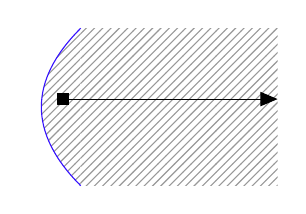
\begin{tikzpicture}
\draw[solid, color={rgb,255:red,53;green,17;blue,254}, pattern=north east lines, pattern color=black!40] (0, 0) to[qcontrol={(-1, 1)}] (0, 2);
\fill[pattern=north east lines, pattern color=black!40] (0, 2) rectangle (2.5, 0);
\draw[square-triangle 45] (-0.3, 1.1) -- (2.5, 1.1);
\end{tikzpicture}
\end{figure}
In which case there are no solutions (note that this case occurs iff $A=0$).
Otherwise, if the ray's origin is outside, there can be $0, 1$ or $2$ intersections. The different cases (where there are $y$-intersections) look as follows:
\begin{figure}[H]
\centering
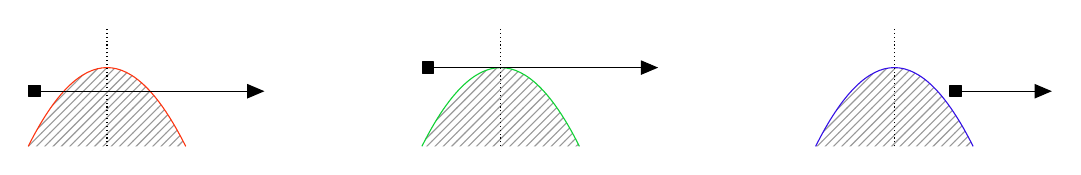
\begin{tikzpicture}
\draw[solid, color={rgb,255:red,254;green,53;blue,17}, pattern=north east lines, pattern color=black!40] (-5, 0) to[qcontrol={(-4, 2)}] (-3, 0);
\draw[solid, color={rgb,255:red,17;green,210;blue,53}, pattern=north east lines, pattern color=black!40] (0, 0) to[qcontrol={(1, 2)}] (2, 0);
\draw[solid, color={rgb,255:red,53;green,17;blue,230}, pattern=north east lines, pattern color=black!40] (5, 0) to[qcontrol={(6, 2)}] (7, 0);
\draw[square-triangle 45] (-5, 0.7) -- (-2, 0.7);
\draw[square-triangle 45] (0, 1) -- (3, 1);
\draw[square-triangle 45] (6.7, 0.7) -- (8, 0.7);
\draw[densely dotted] (-4, 0) -- (-4, 1.5);
\draw[densely dotted] (1, 0) -- (1, 1.5);
\draw[densely dotted] (6, 0) -- (6, 1.5);
\end{tikzpicture}
\end{figure}
Here we can see that if the ray's origin is behind the line through the middle of the curve then all $y$-intersections are true intersections, otherwise none of them are.
One approach to finding whether the ray's origin is inside is by noting that Bézier curves are convex. If we run through the curve the derivative will give us the direction and by rotating that $90^\circ$ we get a normal that always points inwards or outwards. The dot product of this and the vector from the point on the curve to the ray's origin will always have the same sign if the ray's origin is inside, otherwise it will change sign at least once.
This gave a quite complicated expression which could be somewhat simplified to a second-degree polynomial in a single variable, but the discriminant was still to complicated to be calculated exactly on a computer (meaning minimal floating-point arithmetic) due to likely overflow (for 32-bit integers, possibly for 64-bit integers).

Another way to find the intersections is using the resultant, but this resulted in very large expressions. Trying to simplify this via various CAS tools did not yield any improvement (far from that - some even complicated it further). After some experimentation I concluded that this will most likely not give any results.

\end{document}

